\tikzset{
% async
latch/.style={flipflop, flipflop def={t1=D, t6=Q, t3=CLK, 
t4=\ctikztextnot{Q}}},
flipflop SR/.style={flipflop, flipflop def={t1=S, t3=R, t6=Q, 
t4=\ctikztextnot{Q}}},
% sync
flipflop D/.style={flipflop, flipflop def={t1=D, t6=Q, c3=1, 
t4=\ctikztextnot{Q}}},
 flipflop T/.style={flipflop, flipflop def={t1=T, t6=Q, c3=1, 
t4=\ctikztextnot{Q}}},
flipflop JK/.style={flipflop,
flipflop def={t1=J, t3=K, c2=1, t6=Q, t4=\ctikztextnot{Q}}},
% additional features
add async SR/.style={flipflop def={%
tu={\ctikztextnot{SET}}, td={\ctikztextnot{RST}}}},
dot on notQ/.style={flipflop def={t4={Q}, n4=1}},
}


\chapter{Hardware Architecture}

\section{Overview}

\begin{figure}[ht]
    \centering
    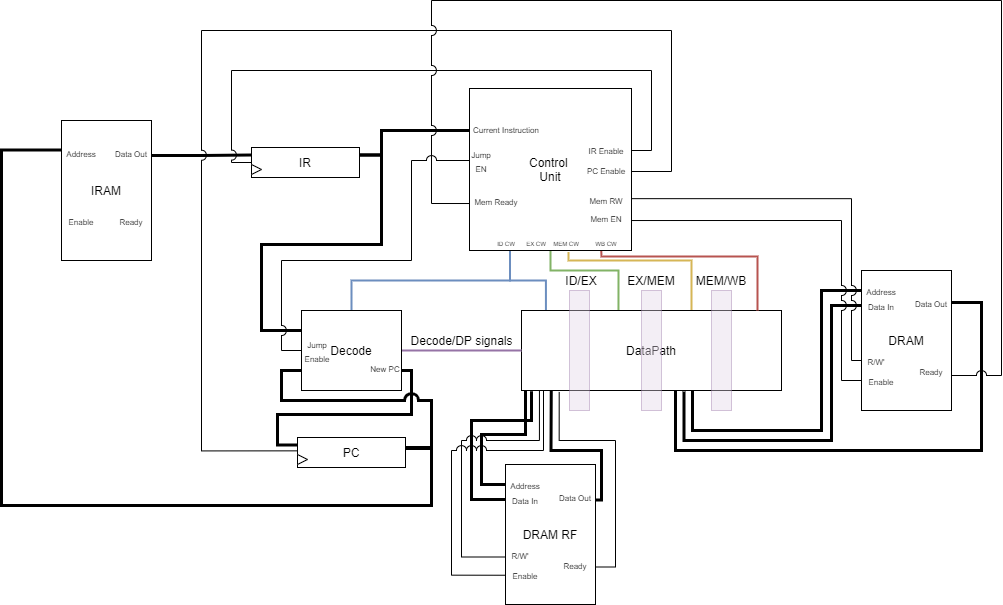
\includegraphics[width=0.9\textwidth]{chapters/2_dlx/images/DLX.png}
    \caption{Schematic of the DLX}
    \label{DLX}
\end{figure} 

\section{Pipeline Stages}
\section{Control Unit}
\section{Memories Interface}
\section{Instruction Set}